\myparagraph{Purpose}
Everytime a special user wants to access to the data of a specific individual it has to pass through some steps:
\begin{enumerate}
  \item It has to insert the SSN of the targeted individual, who will receive a direct request that he/she can accept or refuse;
  \item If the request has been accepted the special user will receive a notification with the payment form with the amount it has to pay to download the required data;
  \item If it pays the amount due it can download the required data.
\end{enumerate}

\myparagraph{Scenario 1}
AC Milan wants to acquire information about the lifestyle of Cristino Ronaldo, so it opens the browser and searches for \textit{Data4Help} web site, it logs in and then it goes in "\textit{Data Search}" area. Then it inserts Ronaldo's SSN, clicks on "\textit{Submit} button and waits a couple of days for a response. Unfortunately, Ronaldo doesn't accept the request, AC Milan receives a notification about the negative response and the process ends.

\myparagraph{Scenario 2}
The "San Gerardo" hospital of Monza is trying \textit{Data4Help} combined with \textit{AutomatedSOS} to monitor the health status of some of its patients after the dismissal. Lucia has been dismissed a couple of month ago and she has \textit{AutomatedSOS} installed on her smartphone. The "San Gerardo" hospital accesses to \textit{Data4Help} from the web site, logs in, goes in "\textit{Data Search}" area, inserts Lucia's SSN, clicks on the "\textit{Submit} button and waits a couple of days for a response. Lucia accepts the request, so the "San Gerardo" hospital receives the notification with the payment form with the amount it has to pay, pays it and downloads Lucia's data.

\myparagraph{Use Case}
The \textit{Individual Data Requirement} use case is analyzed in Table \ref{table:individualDataRequirement}.

\myparagraph{Mockup}
The \textit{Individual Data Requirement} mocukp is shown in Figure \ref{img:individualDataRequirementMockup}.

\myparagraph{Functional requirements}
\begin{enumerate}
  \item The system must refuse a non existant SSN;
  \item The system must not let the special user download the required data untill it hasn't paid the amount due;
  \item The system must send a notification in case of negative response and end the process;
  \item The system must send a notification with the payment form with the amount due in case of positive response;
  \item The system must let the \textbf{Special user} leave the data requirement process at anytime.
\end{enumerate}

\begin{center}
\begin{table}
\begin{tabular}{ | l | p{0.75\linewidth} | }
  \hline
    Actors & \textbf{Special user} and targeted individual \\ \hline
    Goal & \textbf{[G.4]} \\ \hline
    Input Condition & A \textbf{Special user} wants to acquire data of an individual \\ \hline
    Event Flow & \begin{minipage}[t]{0.7\textwidth}
      \begin{enumerate}
        \item The \textbf{Special user} opens the main page of \textit{Data4Help} web site;
        \item The \textbf{Special user} logs in;
        \item The \textbf{Special user} goes in "\textit{Data Search}" area;
        \item The \textbf{Special user} inserts the SSN of the targeted individual;
        \item The \textbf{Special user} clicks on the "\textit{Submit}" button;
        \item The \textbf{Special user} recieves a notification with the response;
        \item If the response is positive the \textbf{Special user} recieves the payment form with the amount it has to pay;
        \item The \textbf{Special user} pays the amount due;
        \item The \textbf{Special user} downloads the required data.
      \end{enumerate}
    \smallskip
  \end{minipage} \\ \hline
  Output Condition & The \textbf{Special user} receives the required data \\ \hline
  Exceptions & \begin{minipage}[t]{0.7\textwidth}
    \begin{itemize}
      \smallskip
      \item If functional requirements 1 is not satisfied the process goes back to step 4;
      \item If functional requirement 2 is not satisfied the process goes back to step 8;
      \item If the targeted individual refuse to share his/her data the process is aborted;
      \item If the \textbf{Special user} decides to leave the data requirement process this one is aborted.
    \end{itemize}
    \smallskip
  \end{minipage}  \\ \hline
\end{tabular}
\caption{\textit{Individual Data Requirement} use case}
\label{table:individualDataRequirement}
\end{table}
\end{center}

\begin{figure}
\begin{center}
  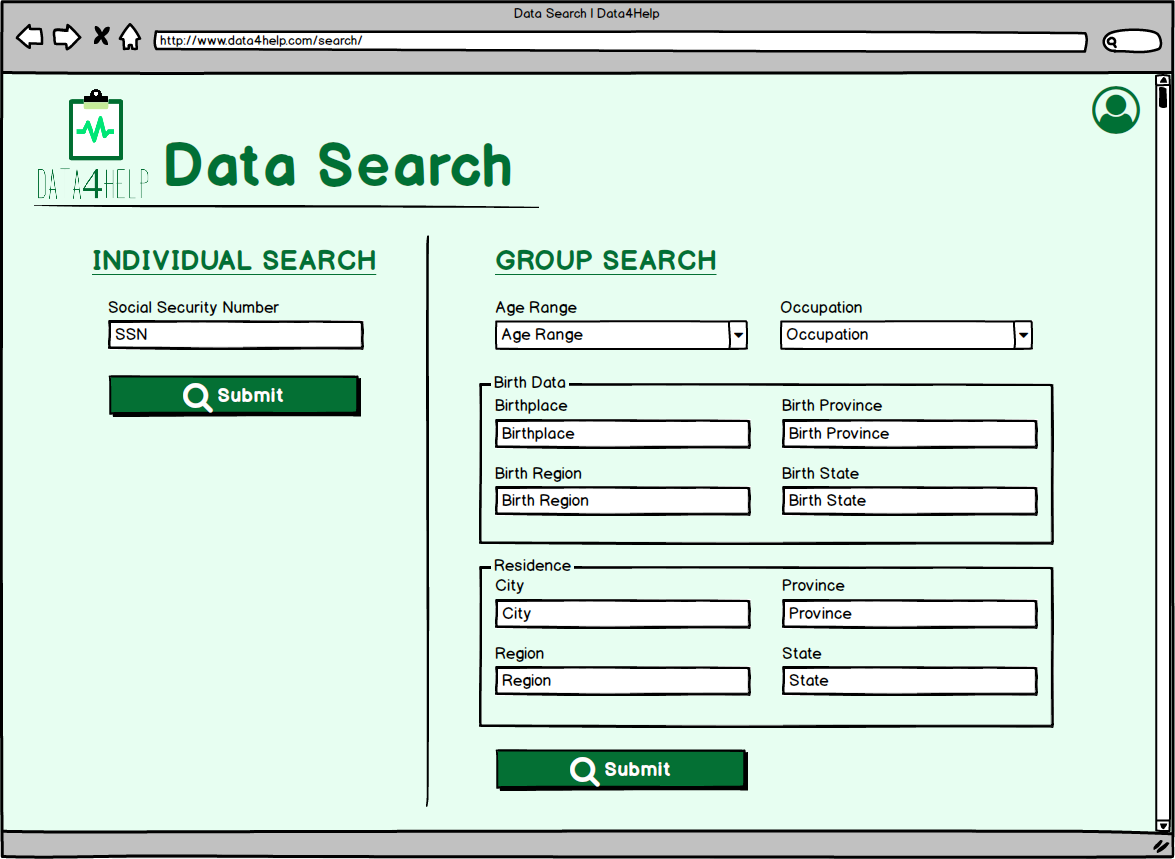
\includegraphics[width=\textwidth]{img/mockup/Data_Search.png}
  \hspace{0.05\linewidth}
  \centering
  \caption{\textit{Individual Data Requirement} mockup}
  \label{img:individualDataRequirementMockup}
\end{center}
\end{figure}
